\documentclass[a4paper]{article}

\usepackage[utf8]{inputenc}
\usepackage[T1]{fontenc}

\usepackage{euler}
\usepackage[OT1]{eulervm}
\renewcommand{\rmdefault}{pplx}

\usepackage{CJKutf8}
\newcommand{\CJKEN}[1]{\begin{CJK}{UTF8}{bkai}#1\end{CJK}}

\usepackage[margin=1in]{geometry}
\usepackage{hyperref}
\usepackage{subfiles}
\usepackage{amsmath,amssymb}
\usepackage{enumitem}
\usepackage{bibunits}

\usepackage{tikz}
\tikzset{
every node/.style={circle, draw=black, inner sep=2pt}
}
\usetikzlibrary{arrows}

\newskip\mt \mt=10pt plus 100pt
\newcommand{\mtskip}{\vspace{\mt}}
\newskip\bt \bt=30pt plus 100pt
\newcommand{\btskip}{\vspace{\bt}}
\newcommand{\talktitle}[1]{{\Large\bf #1}}
\newcommand{\info}[1]{{\footnotesize\tt #1}}

\definecolor{mstitle}{HTML}{193890}
\newenvironment{ilasabstract}{\par\noindent\ignorespaces}{\btskip\ignorespacesafterend}
 
%% \parskip=2cm
%% \parindent=0pt

\title{\bf\Huge The 26th Conference of the\\ International Linear Algebra Society}
\date{}

\pagenumbering{gobble}

\begin{document}

%% SEC: FRONTMATTER
\maketitle

%% \vspace{-4cm}

\begin{center}
% switch lightmode/darkmode by switching black/white in the next line
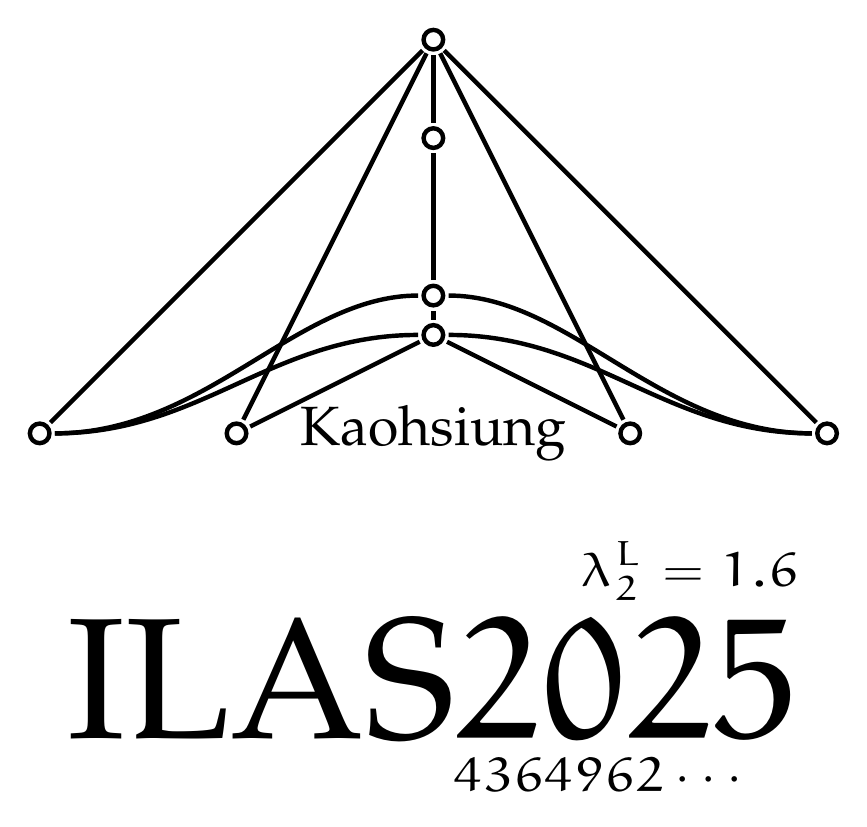
\begin{tikzpicture}[scale=2.5, transform shape, black, 
every node/.style={circle, draw, inner sep=1pt}, 
every label/.style={rectangle, draw=none}]
%% \begin{tikzpicture}[scale=2, transform shape, white]
% help lines
%% \draw[opacity=0] (-2.5,-2.5) grid (2.5,2.5);
%% \node[fill=red] at (0,0) {};

% graph
\begin{scope}[black, ultra thick]
\node (0) at (-2,0) {};
\node (1) at (-1,0) {};
\node (2) at (1,0) {};
\node (3) at (2,0) {};
\node (4) at (0,0.5) {};
\node (5) at (0,0.7) {};
\node (6) at (0,1.5) {};
\node (7) at (0,2) {};

\draw (7) -- (0);
\draw (7) -- (1);
\draw (7) -- (2);
\draw (7) -- (3);
\draw (4) -- (1);
\draw (4) -- (2);
\draw (4) -- (5) -- (6) -- (7);
\draw (4) to [out=180, in=0, out looseness=1] (0);
\draw (4) to [out=0, in=180, out looseness=1] (3);
\draw (5) to [out=180, in=0, out looseness=0.8] (0);
\draw (5) to [out=0, in=180, out looseness=0.8] (3);

\node[draw=none,rectangle] at (0,0) {\footnotesize Kaohsiung};

\end{scope}
% ILAS2025
\begin{scope}[shift={(0,-1.25)}]
\node[rectangle, draw=none] (ILAS2025) at (0,0) {\Huge ILAS$2025$};
\node[rectangle, draw=none, above, xshift=1.3cm] at (ILAS2025.north) {\scriptsize$\lambda_2^L = 1.6$};
\node[rectangle, draw=none, below, xshift=0.86cm] at (ILAS2025.south) {\scriptsize$4364962\cdots$};

\end{scope}
\end{tikzpicture}
\end{center}

\begin{LARGE}
\begin{center}
\vfil

June 23 $\sim$ 27, 2025 $\infty$ Kaohsiung, Taiwan

\vfil

National Sun Yat-sen University
  
\end{center}
\end{LARGE}

\newpage

%% SEC: BCAKMATTER

\begin{center}
\makebox[0pt]{
\begin{tikzpicture}[every node/.style={draw=none,rectangle}]
\node at (0,0) {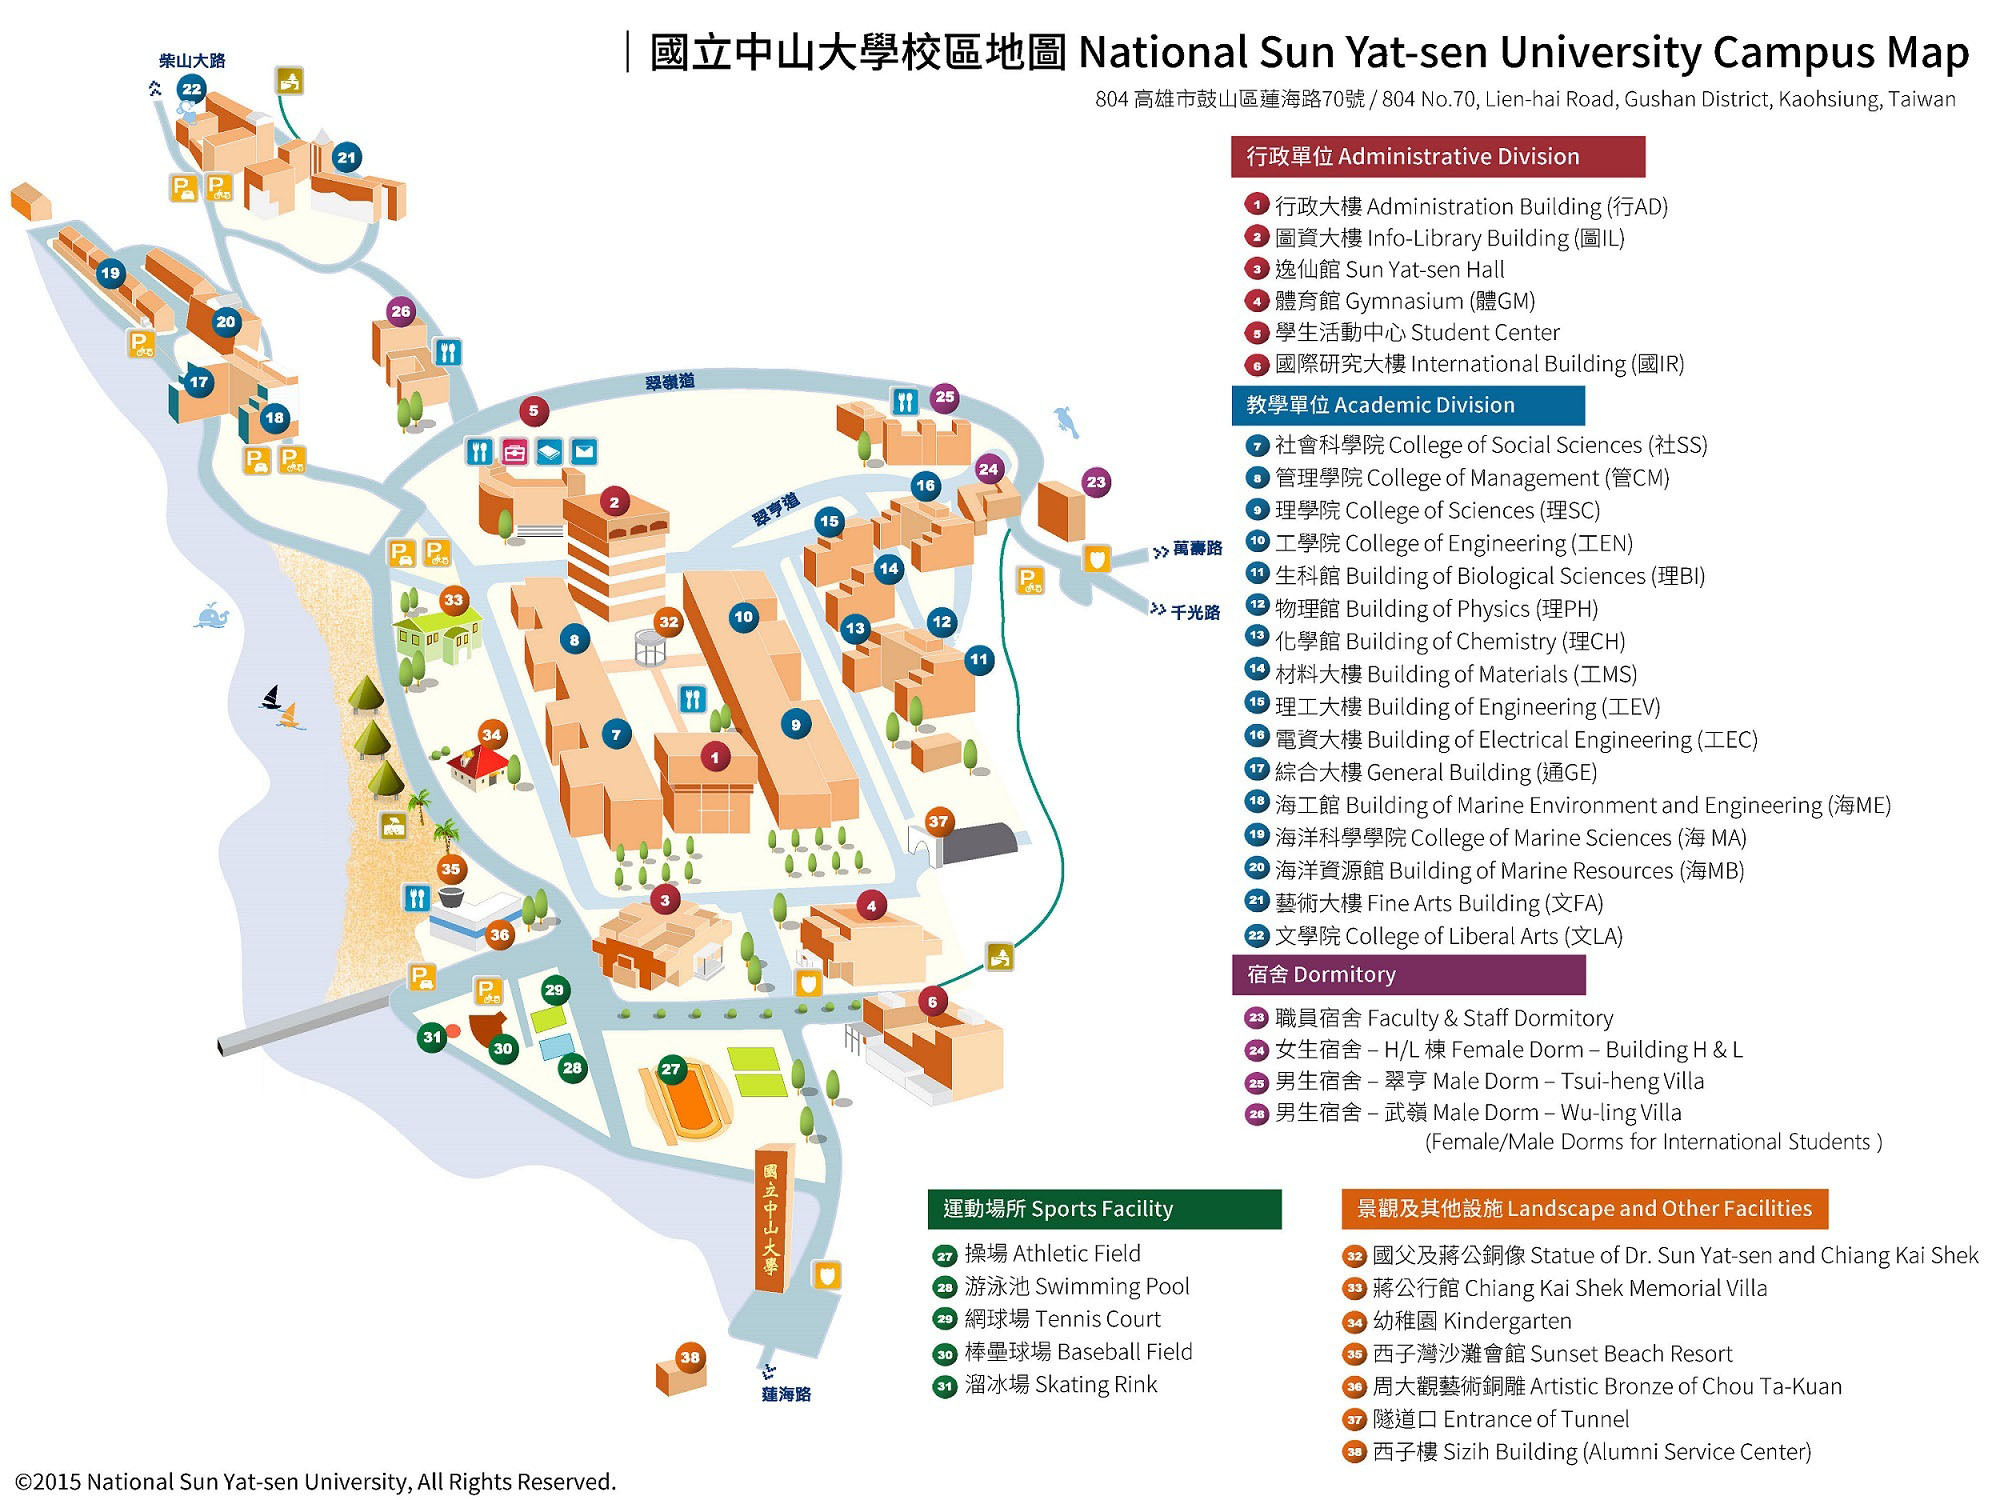
\includegraphics[scale=1.2]{logomap/MAP2018-en}};
%% \node[draw=black] at (0,0) {};
%% \draw (-6,-3) grid (6,3);

\begin{scope}[very thick, every node/.style={draw=black, inner sep=5pt, circle}]
\node (ms) at (-2.06,0.27) {};
\node[draw=none, rectangle, align=center] (ms-text) at (-2,5) {\bf\sf\large College of Science\\(Mini-symposia)};
\draw[->] (ms-text.south) -- (ms.north);

\node (sys) at (-3.39,-1.5) {};
\node[draw=none, rectangle, align=center] (sys-text) at (-9,0) {\bf\sf\large SYS Hall\\(Plenary)};
\draw[->] (sys-text.south east) -- (sys.west);

\node (sun) at (-7,-2.75) {};
\node[draw=none,rectangle] (sun-text) at (-7,-5) {\bf\sf\large Sunset view};
\draw[->] (sun-text.north) -- (sun.south);
\end{scope}
\end{tikzpicture}
}
\end{center}

\vfill
\hrule
\vspace{2pt}
\begin{center}
%%% SINICA
%% \begin{tikzpicture}[every node/.style={draw=none,rectangle}]
%% \node[left] at (0,0) {\includegraphics[scale=0.2]{logomap/AS-grayscale}};
%% \node[right,align=left] at (0,0) {\sf\large Institute of Mathematics\\ \sf\large Academia Sinica};
%% \end{tikzpicture}
%% \hfil
%%% MRPC
%% \begin{tikzpicture}[every node/.style={draw=none,rectangle}]
%% \node[left] at (0,0) {\includegraphics[scale=0.18]{logomap/MRPC-grayscale}};
%\node[right,align=left] at (0,0) {\sf\large Mathematics Research Promotion Center};
%% \end{tikzpicture}
%% \end{center}
%% \begin{center}
%% \hfil
%%% NSYSU
%% \begin{tikzpicture}[every node/.style={draw=none,rectangle}]
%% \node[left] at (0,0) {\includegraphics[scale=0.03]{logomap/NSYSU-grayscale}};
%% \node[right,align=left] at (0,0) {\sf\large National Sun Yat-sen \\ \sf\large University};
%% \end{tikzpicture}
%% \end{center}
%%% MOST
%% \begin{center}
%% \begin{tikzpicture}[every node/.style={draw=none,rectangle}]
%% \node[left] at (0,0) {\includegraphics[scale=0.6]{logomap/MOST-mono}};
%% \node[right,align=left] at (0,0) {\sf\large Ministry of Science and Technology};
%% \end{tikzpicture}
\end{center}

\newpage

%% SEC: TOC
\tableofcontents

\newpage

\pagenumbering{arabic}

\subfile{schedule}

\subfile{abstract}

%% \subfile{content}

%%% Add 6 blank pages
%% \foreach \i in {1,...,6}{
%% \newpage
%% \begin{center}
%% \begin{tikzpicture}[every node/.style={draw=none,rectangle}]
%% \node[opacity=0.5] at (0,0) {\huge Notes};
%% \end{tikzpicture}
%% \end{center}
%% }

\end{document}

%> \thebibliography=\long macro:
%#1->\section *{\refname }\@mkboth {\MakeUppercase \refname }{\MakeUppercase \refname }\list {\@biblabel {\@arabic \c@enumiv }}{\settowidth \labelwidth {\@biblabel {#1}}\leftmargin \labelwidth \advance \leftmargin \labelsep \@openbib@code \usecounter {enumiv}\let \p@enumiv \@empty \renewcommand \theenumiv {\@arabic \c@enumiv }}\sloppy \clubpenalty 4000 \@clubpenalty \clubpenalty \widowpenalty 4000\sfcode `\.\@m .

